% Carsten: 
% I don’t like the flow of 6.1.
% That it because it reads like “I put from several prefab components together and then I did gesture recognition with the Leap Motion. 
% While you may actually yourself feel like that’s what you’ve done, you should not write it like that.
% 
% In section 1, show the design of the bigger picture. How is it imagined (referring to new chapter between 1 and 2) that a approval engineer 
% will work. Sit at a desk, optionally using Oculus and/or Leap but also regular keyboard and screen. Access a design (may be through loading) and 
% interact with it. Make annotations (versioned), store and share them. Find them again later. Perhaps support a cooperative mode.
% 
% Followed by section 2, where you clarify the focus on interaction, and the need for an implementation of a system for testing purposes. 
% You needed loading, rendering, obviously, in addition to navigation and interaction. At the core of your system is the Unity engine, so start with this. 
% Why Unity? Repeat that other things can be connected in a straightforward manner. Mention the loader code.
% 
% The ship model itself should receive a bit of attention in chapter 7.

% \section{External Assets}
% \label{sec:external_assets}
% \import{}{external_assets.tex}

\section{The architecture}
\begin{figure}%[h!] %[H]
	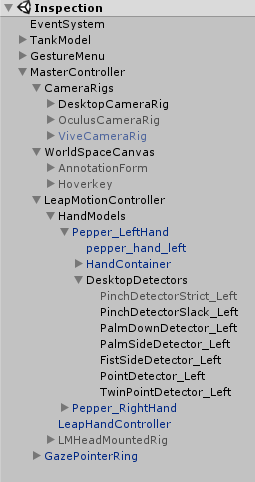
\includegraphics[width=\linewidth]{pictures/unity_hierarchy.png} % Create a better hierarchical view?
	\caption[The Unity project hierarchy of the Design Review Application]{The Unity project hierarchy of the Design Review Application}
	\label{fig:unity_hierarchy}
\end{figure} 

This chapter will document the implementation of the design review application, which was conducted according to the design - discussed in chapter~\ref{chapter:design} - 
and utilizes many of the components reviewed in the technical review (chapter~\ref{chapter:technical}). The application is envisioned to be used by DNV GL Approval Engineers 
(discussed in chapter~\ref{chapter:dnvgl}), which are responsible for reviewing design proposals in the form of complex 3D models and communicate their finding - whether it 
be general information or reporting errors - to the designer. The designer then have to fix any shortcomings reported by the Approval Engineer before again submitting 
his or her 3D model for approval. With the design review application, the Approval Engineer and designer could achieve this, and more, directly in the application.
In this thesis implementation annotations can be stored in the model, edited, deleted and their appearance can be manipulated. The user is also able to navigate the 
3D model using only gesture, only keyboard and mouse, or a combination of the two.

The design review application is designed to primarily be used at a regular workspace, containing a computer and - optionally - a Leap Motion and a virtual reality headset.
The user should thus be able to use the application without any virtual reality or gesture recognition peripherals, only with one of them (i.e a VR HMD or a Leap Motion Controller) 
or with both of them. When using the application the user will thus always have keyboard and mouse available as an input method, 
and can thus use these in combination with the Leap Motion Controller. If the application is started with a virtual reality HMD connected the application will also be displayed
both on the HMD's lenses and on the desktop display, although certain settings - such as the field of view - is affected by the presence or absence of a VR HMD. 

This chapter will primarily document how the implementation is organized as a Unity project, what the major components are, and how it performs its most important functions
(such as recognizing gestures and creating annotations). When the implementation was completed, and thus had fulfilled the functional demands from the design, 
the application was tested and evaluated by DNV GL employees to gain feedback for continued development. This evaluation, and the participants responses are 
covered in chapter~\ref{chapter:evaluation}.

\section{The Project Organization}
The Unity project has four top-level game objects: \texttt{EventSystem}, \texttt{TankModel}, \texttt{GestureMenu} and \texttt{MasterController}. 

The \texttt{EventSystem} game object is responsible for processing and handling events and input actions in the scene. 
In this implementation a standard unity event system is used (generated when creating a new project), with some modifications done for virtual reality.
Most of these modification are accomplished by the attached \texttt{OVRInputModule} script, which is a script inspired by a similar one in an Oculus VR sample project. 
Apart from this no other changes was done to \texttt{EventSystem} as it worked optimally "right out of the box".

The \texttt{TankModel} game object contains several child objects that together make up the oiltank-model, which this application is based on.
Originally the design included the functionality to load different models into the application and starts sessions, but 
this fell out of scope to both prioritize the gesture recognition and virtual reality aspects, and because of a low availability of similar models.
The tanker model has not received any changes during implementation and has been used as it was supplied. 

The \texttt{GestureMenu} and \texttt{MasterController} together contain most of the key components of the application and will, with their relevant child objects,
be the main focus for the rest of this chapter. \texttt{GestureMenu} represents the gesture menu, which by default is available by directing the left hand palm in the 
direction of the camera. The \texttt{MasterController} game object represents the \textit{player model} - i.e the user's virtual presence in the model - 
and has many important game objects as children, in addition to holding many key scripts. 
The \texttt{MasterController}'s transform, with its position, rotation and scale, represents the user's position and orientation, 
and every child object of \texttt{MasterController} will have a position, rotation and scale that is relative to its own. This ensures
that e.g.~the camera and hand models will always "follow" the user. Several of the important game objects that are covered in later sections are children of 
the master controller for this reason. First, however, we will cover the important components of \texttt{MasterController}.
Note that several times during this documentation we will discuss "the cameras" - in plural - as the implementation always utilizes two or more cameras simultaneously, 
even through they appear as one to the user. This will be expanded upon in section~\vref{sec:camera_rigs}.

\begin{figure}%[h!] %[H]
	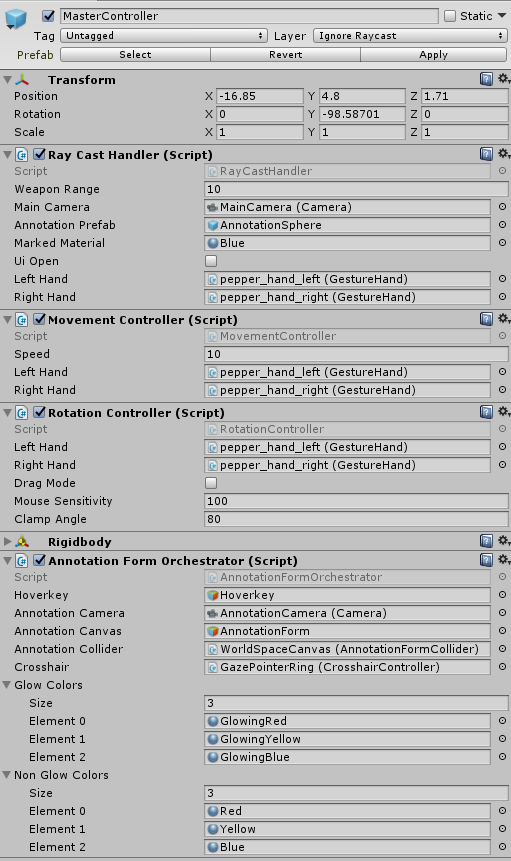
\includegraphics{pictures/unity_inspector.png} % Get better resolution?
	\caption[The \texttt{MasterController} components]{The \texttt{MasterController} components seen in the Unity Inspector view.}
	\label{fig:unity_inspector}
\end{figure} 

\section{The Master Controller Components}
\import{}{master_controller_components.tex}


\section{The Camera Rigs}
\label{sec:camera_rigs}
\import{}{camera_rigs.tex}


\section{The World Space Canvas}
\label{sec:world_space_canvas}
\import{}{world_space_canvas.tex}


\section{The Leap Motion Controller}
\label{sec:leap_motion_controller}
\import{}{leap_motion_controller.tex}


\section{The Gesture Hand Class}
\label{sec:gesturehand_class}
\import{}{gesturehand_class.tex}
 

\section{The Detectors}
\label{sec:detectors}
\import{}{detectors.tex}


\section{The Menu}
\label{sec:menu}
\import{}{menu.tex}


\section{The Annotations}
\label{sec:annotations}
\import{}{annotations.tex}


%\section{Summary}
